\chapter{Contexte du stage}

Intro

\section{Entreprise}

\subsection{Presentation générale }
Néréide est une société de services en logiciels libres crée en 2004 qui se spécialise dans l'intégration du progiciel de gestion intégré Apache OFBiz. Il s'agit d'une société coopérative et participative (SCOP) qui se situe à Tours. 



\subsection{Activité}
\label{activite}
Transparence libre entreprise \\


Integration(utilisation des briques en tant que telles) et
Dévéloppement spécifique (adaptation d'OFBIZ pour les besoins ) plugins propres à la logique métier. Pas de forfait(contrat doit etre rempli, l'entreprise s'engage à ce qu'il soit livré dans les tepms), mais la régie (sont payé au temps de travail et pas à condition de remplir un contrat ).  Pareil avec Décath 6 pers font de la régie...
Administration système
\subsection{Projets}
\subsubsection{Décathlon}
L'un des principaux clients de Néréide est le groupe Decathlon qui se spécialise en grande distribution de produits de sport et de loisirs. 
Le projet représente une plateforme de vente de puces RFID(bookmark), qui assure l'intégralité du processus d'achat.

pour les achteurs et producteurs, dev front pour le store specifique au lieu d'écrans OFBiz, communication avec des API...

\subsubsection{Déjbox}

Dejbox est une société de la foodTech qui propose aux salariés d’entreprise de leur livrer des repas directement sur leur lieu de travail. L’ensemble des vente est réalisé au travers d’un site e-commerce par lequel le salarié commande un repas.

Le projet a pour objectif de mettre en œuvre un outil de type ERP afin de gérer la chaîne de réapprovisionnement en produit frais vendu en ligne. Il s’agit donc de créer un référentiel d’article et de fournisseur et de pouvoir saisir des commandes qui seront envoyées aux fournisseurs et réceptionnées suite à leur livraison. Enfin, il s’agit de mettre en place la sortie de stock en intégrant les consommations de produit provenant du site de vente en ligne.


....
Dépuis 2013 les dev remontantes à la communauté , parce que besoin de support,  divergence. moutons-acteur 







\section{Framework OFBiz}
\subsection{Vue d'ensemble }
\emph{Open For Business (OFBiz)} est une suite d'applications pour la gestion de l'entreprise qui se base sur une architecture très couramment utilisé \emph{(MVC)} et qui implémente des composantes classiques de gestion des donnés, de logique métier, et de traitement spécialisé. 

On peut notamment distinguer les modules génériques destinées à la gestion des tâches communes à la plupart des entreprises, telles que la gestion des stocks, la comptabilité, la facturation et bien d'autres. Quant à leur structure, toutes les composantes sont étroitement liées entres elles, ce qui facilite la compréhension, l'utilisation et la personnalisation de ces dernières. 


En plus d'une architecture qui encourage la customisation, OFBiz est entièrement distribué en tant que \emph{open source software}\footnote{Logiciel libre sous licence \href{https://www.apache.org/licenses/LICENSE-2.0.html}{ASL2 (Apache License Version 2.0)} ce qui donne le droit de personnaliser, d'étendre, de restructurer et de vendre le système concerné. } ce qui le rend particulièrement intéressant car le logiciel développé à base de OFBiz n'est pas soumis à la condition d'être libre comme c'est le cas de la licence GPL  \footnote{\href{http://www.gnu.org/licenses/gpl-3.0.html}{GNU General Public Licence}} par exemple.

\subsection{Architecture }
D'un point de vue purement technique OFBiz se base sur la plateforme Java ainsi que sur l'utilisation des DSL\footnote{Domaine specific language \emph{(Langages spécifiques au domaine)}} basés sur des grammaires écrites en XML (mettre la bib). En ce qui concerne la partie principale du framework, les échanges HTTP sont implémentes par une extension de la classe \verb=HTTPServlet= \cite{chan2017servlet} et la communication avec les bases de données se fait via l'API Java JDBC \cite{JDBC}.

Dans sa structure on distingue \emph{le framework}, \emph{les applications} et \emph{les plugins}. Le \emph{framework} comporte l'ensemble des outils et des mécanismes techniques de bas niveau utilisés par les applications. Il fournit notamment des fonctionnalités présentes dans la plupart des frameworks de développement(couche données, logique métier,gestion des transactions, etc...).
Les principaux composants métier tels que la comptabilité, la gestion des stock, ou la facturation se trouvent dans la partie \emph{applications}. 
Finalement la notion du plugin  correspond à une application spécifique qui repose sur des composantes générales: par exemple le plugin \emph{eCommerce} correspond à un boutique en ligne interagit avec des nombreuses  \emph{applications} comme \emph{la gestion du stock} ou \emph{la facturation}. 

\subsection{DSL XML}
L'une des particularités d'OFBiz ce sont des fichiers XML qui servent à déclarer entre autres
des routes HTTP, des pages de rendu appelés \emph{Écrans}, ainsi que des services. Le principe est de transformer des informations sous format XML facilement compréhensibles par le développeur, en objets Java correspondants. 


\definecolor{dollarbill}{rgb}{0.52, 0.73, 0.4}
\subsection{Container}
L'interface container représenté sur la figure \ref{container} permet de définir des objets qui correspondent à des processus qui peuvent être initialisés, démarrés et arrêtés. L'intérêt est de pouvoir lancer un daemon spécifique en parallèle de l'execution d'OFBiz comme c'est le cas de \verb|EntityDataLoadContainer| qui est responsable du chargement des données et leur mise à jour en cas de modification du modèle. Quand à \verb|TestRunContainer| il s'assure du lancement des testes unitaires grâce à un mécanisme propre au framework. 
\begin{figure}[h!]
	\centering
	\begin{tikzpicture}
	\umlinterface[scale=0.8,x=0,y=5]{Container}{}{
		\umlvirt{+ init(cmds : List<StartupCommand>, name : String,} \\
		\umlvirt{\hspace{1,1cm}config : String) : void} \\
		\umlvirt{+ start() : void} \\
		\umlvirt{+ stop() : void} \\
		\umlvirt{+ getName() : String}
	}
	\umlclass[ x=-5, y=-1,scale=0.8]{EntityDataLoadContainer}{
		- name : String \\
		- module : String
	}{
		\umlvirt{+ getName() : String} \\
		\umlvirt{+ createDbConstraints(...) : void}\\
		\umlvirt{+ dropPrimaryKeys(...) : void}
	}
	\umlclass[ x=6, y=-1,scale=0.8]{TestRunContainer}{
		- name : String \\
		- jsWrapper : JunitSuiteWrapper
	}{
		\umlvirt{+ getName() : String} \\
		\umlvirt{+ createJunitXmlListener(...) : JunitXmlListener} \\
		\umlvirt{+ logTestSuiteResults(...) : void} \\
	}

 \umldep[geometry=|-|, pos1=1.5, pos2=0.2 ,draw=dollarbill,  thick]{TestRunContainer}{Container}
 \umldep[geometry=|-|, pos1=1.5, pos2=0.2 ,draw=dollarbill,  thick]{EntityDataLoadContainer}{Container}
	\end{tikzpicture}
	
	
	\caption{Définition du type container}
	\label{container}
\end{figure}
\subsection{Composants}
Les éléments constitutifs de OFBIZ sont des composants. Un composant est un regroupement des containers, des entités, des services, des vues (\emph{Écrans}) et des applications Web.


L'exemple classique d'un composant est celui de \verb|webtools| qui assure la gestion technique de l'ensemble du système par l'administrateur via une application web, ce qui implique le fait que ce composant regroupe la plupart des éléments majeurs du framework.
Nous en tant que développeurs avons la possibilité de définir nos propres composants, notamment des \emph{plugins}. 
  


\subsection{Web applications}
Des composant OFBiz ne peuvent pas être accédés directement par les utilisateurs, ils servent simplement à organiser le framework en parties individuelles de chaque aspect de l'ERP afin de faciliter leur gestion. Les applications web \emph{(webapps)} sont destinées à fournir un front-end afin que les utilisateurs puissent interagir avec OFBiz. En ce qui concerne les routes HTTP, définis classiquement dans le fichier \verb|web.xml|, dans le cas de OFBiz leur gestion est délégué à un ficher \verb|controller.xml| qui à son tour associe des traitement spécifiques à chaque point d'entrée HTTP ainsi que la valeur de retour qui peut être une vue \emph{(Écran)}, du type \verb|JSON| ou bien une redirection. Cela se fait au moyen d'une \verb|request-map| comme on peut voir sur l'extrait de code suivant \ref{reqmap}



\lstset{language=XML}
\begin{figure}
\begin{lstlisting}
<request-map uri="stock">
    <event type="service" invoke="getStock"/>
    <response name="success" type="view" value="stockScreen"/>
</request-map>
\end{lstlisting}
	\caption{Association d'un point d'entrée et d'une réponse}
\label{reqmap}
\end{figure}



\subsection{Entity engine}
Comme dans beaucoup d'autres frameworks, l'interaction avec les bases de données à une place principale dans le OFBiz. Le moteur d'entités (\emph{Entity engine}) se charge de la communication avec les  bases de données à travers les déclarations uniformes, c'est à dire qui changent pas peu importe le choix de l'outil externe de gestion.



\subsection{Service engine}
Les services web assurent les échanges d'information être les applications, communément via le protocole\verb| HTTP|.   
Les services OFBiz fonctionnent dans une architecture orientée service (SOA). Non seulement ces services ont une capacité d'évoquer les autres intérieurement, mais peuvent aussi être appelés par une application extérieure en utilisant des protocoles d'échange d'information tells que \verb|SOAP|. 

Les services OFBiz sont appelées en passant un contexte \footnote{Définis souvent dans les paramètres de la requête HTTP } et retournent une réponse parmi celles conventionnellement nommés: \emph{"success"}, comme on peut voir dans  \ref{reqmap} , \emph{"error"} ou \emph{"failure"} ainsi que l'ensemble des données retournées par le service. 

On peut voir l'exemple de la définition d'un service sur \ref{servicedef} , qui montre notamment la saisie des attributs attendu par le service qui sont définis de deux manières: En utilisant le mécanisme de \verb|auto-attributes| qui génère des attributs\footnote{Qui sont en l'occurence en entrée (de paramètre IN)} à partir de l'ensemble des clés primaires de l'entité \verb|Stock|. L'autre manière de faire est de rajouter des attributs manuellement comme on peut le voir dans la suite de l'exemple. 


\begin{figure}
\begin{lstlisting}
<service name="getStock" engine="entity-auto" default-entity-name="Stock">
  <auto-attributes include="pk" mode="IN" optional="false"/>
  <attribute name="authKey" type="String" mode="IN" optional="true"/>
  <attribute name="stockList" type="String" mode="OUT" optional="true"/>
</service>
\end{lstlisting}
\caption{Définition d'un service}
\label{servicedef}
\end{figure}


\subsection{Screen engine}
La partie Vue du MVC est représentée par des \emph{Écrans} ou les \verb|Screen| qui font partie du \verb|Widget toolkt| \footnote{Boite d'outil de composant d'interface graphique} de OFBiz. Le principe du fonctionnement d'un écran se base toujours sur un DSL qui interagit avec un mécanisme de rendu générique capable de gérer différents formats de sortie comme \verb|HTML|, \verb|XML|, \verb|CSV|, ou \verb|XLS|. Le cas d'utilisation le plus commun est celui d'une réponse HTML qui est éventuellement générée en déléguant le rendu à un autre mécanisme : \verb|Apache Freemarker|.
\begin{figure}[h!]
	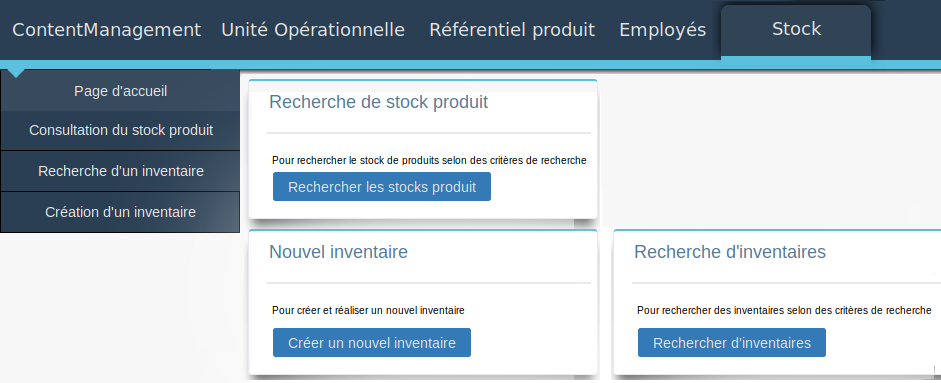
\includegraphics[width=\linewidth]{screenOfbiZ.png}
	\caption{L'exemple d'un Ecran de rendu OFBiz.}
	\label{fig:screen}
\end{figure}

\subsection{Fonctionnel métier}
Le méta-composant \emph{Applications} comporte des composants métier prédéfinis, qui ont pour vocation de fournir des solutions fonctionnelles "prêtes à l'emploi". 

Ainsi on distingue parmi d'autres :
\begin{labeling}{alligator}
	\item [\textbf{accounting}] fournit l'ensemble de services et d'écrans de rendu pour la comptabilité.
	\item [\textbf{datamodel}] s'occupe de la définition des entités et des relations entre elles.
	\item [\textbf{humanres}] correspond à la gestion du personnel.
	\item [\textbf{product}] permet la gestion du catalogue des produits et des services fournis par l'organisme.
\end{labeling}


\section{Sujet de stage }
Comme mentionné avant, le sujet de stage est divisé en deux parties. La première partie consiste à prendre en main l'outil de développement concerné, le framework OFBiz. La deuxième partie du stage est la modification de certains éléments du framework, notamment des mécanismes de gestion de services afin d'assurer la conformité au style architectural REST.  

\subsection{Découverte OFBiz}
Cette étape sert à se familiariser avec l'environnement du framework à travers des tutoriels et l'analyse des projets existants, afin de comprendre le fonctionnement général. Cela permet aussi de repérer les points essentielles auxquelles il faut tenir compte lors de la deuxième phase de travail. 

\subsection{API REST au sein d'OFBiz}

Finalement, l'intérêt principal du stage est la mise en place d'un système de gestion des services REST. L'idée a été évoquée pour la première fois dans une \href{https://issues.apache.org/jira/browse/OFBIZ-4274}{discussion communautaire} Apache OFBiz, car le mécanisme en cours nécessitait de l'évolution. Cette discussion a suscité des nombreuses remarques en terme de faisabilité et a permis de retrouver des pistes à poursuivre lors de l'implémentation.  

Dans un premier temps on considère la possibilité d'intégration d'une solution externe notamment à travers des librairies JAX-RS de CXF, ainsi que Apache Camel. Malgré les premières prototypes fonctionnelles l'idée d'une solution externe a été abandonné pour des raisons expliqués plus loin dans le document. A sa place une implémentation de bas niveau a été adoptée. Une fois le système mis en route, l'étape suivante consistait à faire adopter la modification dans la branche principe du projet OFBiz. 

Afin de prouver la conformité du nouveau système et démontrer les nouveaux fonctionnalités, la décision a été prise de modifier une partie front-end existante, notamment l'interface de gestion des entités \emph{entitymaint}. Finalement, l'ensemble de modification sous la forme des patchs a été soumis à la communauté afin d'être revus et potentiellement adoptés dans le framework. 









